%Первоочерёдной задачей при анализе влияния микролинзирования на кривые блеска SN Refsdal является оценка параметров галактики-линзы, ответственной за появление изображений S1-S4 (см. Рис. \ref{fig:snrefsdalfig}). На основе эмпирических соотношений для основных свойств эллиптических галактик - эффективного радиуса $r_e$, эффективной поверхностной плотности $\Sigma_e$ и дисперсии скоростей звёзд $\sigma_{prox}$ (\cite{schechter2014}, - а также закона де Вокулёра (\cite{vaucouleurs}), который связывает поверхностную яркость в эллиптической галактике с расстоянием до её центра, была проведена оценка $\kappa*$, $\kappa_c$ и $\gamma$ в областях, в которых находятся изображения S1-S4 SN Refsdal, координаты которых относительно центра эллиптической галактики известны из работы \cite{kawamataoguri}, и на основе этого построены карты усилений для этих областей. Детальный вывод вышеупомянутых параметров представлен в Приложении. \textbf{Или лучше пусть здесь будет?} 

%Локальные значения параметров $\kappa_*, \kappa_c$ и $\gamma$ в областях изображений S1-S4 представлены в Таблице \ref{tab:allparamsfors1234}.

%\begin{table}[H]
%  \caption{Оценки параметров для изображений SN Refsdal}
%   \label{tab:allparamsfors1234}
%  \centering
%    \begin{tabular}{ | c | c | c | c | c |}
%    \hline
%    Изображение & S1 & S2 & S3 & S4 \\ \hline
%    $\kappa$ & 0.728 & 0.725 & 0.670 & 0.744 \\ \hline
%    $\gamma$ & 0.108 & 0.347 & 0.221 & 0.484 \\ \hline
%    $\Sigma_*, M_{\odot}/pc^2$ & 491.2 & 541.3 & 509.8 & 580.1\\ \hline
%    $\kappa_*$ & 0.207 &  0.228 & 0.215 & 0.245 \\ \hline
%    $\kappa_c$ & 0.521 & 0.496 & 0.455 & 0.499 \\ \hline
%    $\kappa_*/\kappa$ & 0.285 & 0.315 & 0.321 & 0.329 \\ \hline
%    \end{tabular}
%\end{table}

В данной работе анализируются кривые блеска SN Refsdal, наблюдаемые в изображениях S1 и S2, так как временная задержка между ними рассчитана с наименьшими погрешностями. Для набора параметров, характеризующих области этих изображений, в программе \texttt{microlens} построены карты микролинзирования. Они изображены на Рисунке \ref{fig:mymaps}, размер каждой карты - $5\times5$ радиусов Эйнштейна в плоскости источника, разрешение - $10000\times10000$ пикселей. Выбор такого масштаба (1 радиус Эйнштейна = 2000 пикселей) обусловлен необходимостью задания профиля яркости сверхновой на большом количестве точек вдоль радиуса. В рамках проверки корректности полученных карт проведено их статистическое исследование. Гистограммы по их значениям сравниваются с гистограммами карт с аналогичными параметрами из обзора \texttt{GERLUMPH} (\cite{gerlumph}). Эти карты получены независимой командой исследователей и лежат в открытом доступе. Кроме того, на гистограммы также нанесена зависимость $\mu^{-3}$, которой подчиняется усиление точечных источников для больших $\mu$ (\cite{wambsganss1992-probabilities}, \cite{blandfordnarayan1986}). Максимальный радиус SN Refsdal на этих картах – 72 пикселя. Предполагается, что при таком масштабе станет возможным различить флуктуации микролинзирования от источников с плоским и гауссовым профилями яркости. На Рисунке \ref{fig:mymaps} изображены полученные карты и построенные по ним гистограммы. Светлые области означают, что точечный источник усиливается, находясь в них, тёмные - что ослабляется. Видно, что а) сеть каустик отличается в зависимости от входных параметров, б) практически по всей карте усиление меняется и почти нигде не остаётся таким, каким его предсказывает модель линзы, то есть в отсутствие микролинзирования.

\begin{figure}[H]
    \centering
	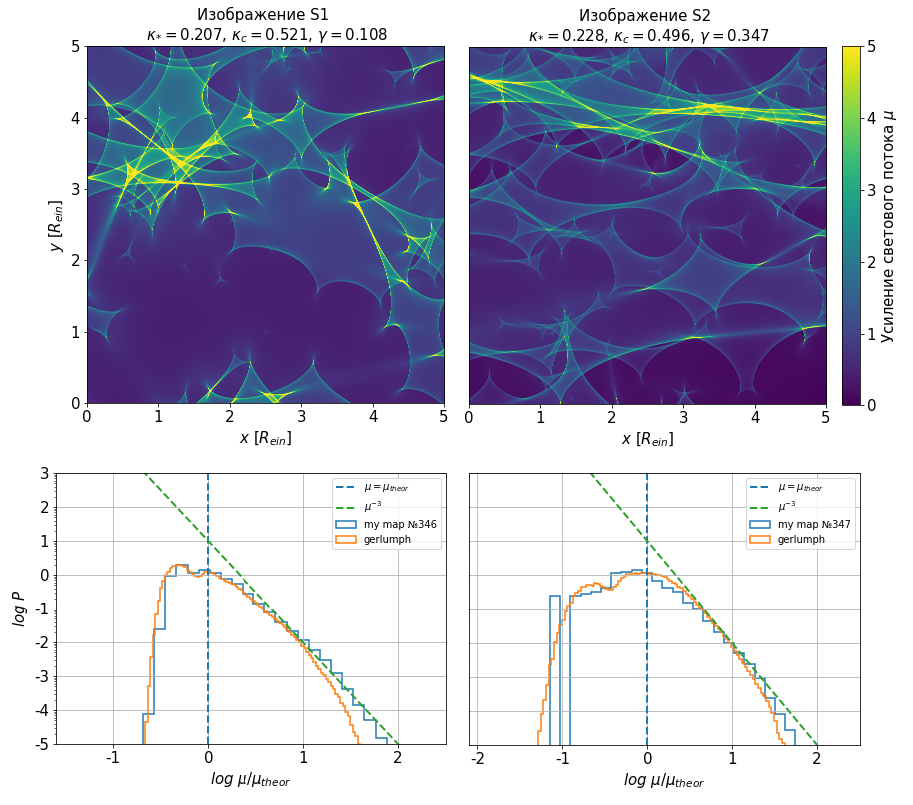
\includegraphics[width=\textwidth]{microlensing/images/mapsandhistS12.png}
	\caption{Сверху: Карты усилений, вызванных микролинзированием, в областях изображений S1 (слева) и S2 (справа) SN Refsdal. Значения усилений ограничены сверху для контраста, в действительности в некоторых областях значение абсолютных усилений может достигать нескольких десятков. Снизу: гистограммы по этим картам и по картам из обзора GERLUMPH с теми же параметрами. На гистограммы нанесена теоретическая вероятность $P(\mu)\propto \mu^{-3}$ в пределе больших усилений $\mu$ (зелёная пунктирная линия) и теоретическое значение усиления в отсутствие микролинзирования (синяя пунктирная линия).}
	\label{fig:mymaps}
\end{figure}


Теоретическое макро-усиление карты (другими словами, среднее усиление по карте) зависит от параметров $\kappa$ и $\gamma$ и определяется ранее указанной формулой:

\begin{equation}\tag{\ref{eq:magnification}}
\mu_{th} = \frac{1}{(1-\kappa)^2-\gamma^2}.
\end{equation}

Среднее численное усиление карты задаётся формулой

\begin{equation}\label{avmag}
\mu_{num} = \frac{1}{N_{pix}^2}\sum_{i,j=1}^{n_{pix}}\mu_{ij} \ ,
\end{equation}

\noindent где $N_{pix}$ - сторона карты в пикселях, $\mu_{ij}$ - усиление пикселя с координатами $(i,j)$. Значения $\mu_{th}$ и $\mu_{num}$, как правило, в точности не равны друг другу, так как параметры, по которым построена карта, описывают гораздо большую область, чем та, для которой эта карта построена. Таким образом, средняя поверхностная плотность массы внутри региона, для которого построена карта, может быть больше или меньше, чем та что использовалась в качестве входного параметра. Кроме того, численное и теоретическое усиление могут не совпадать в силу того, что характерный размер некоторых каустик больше, чем размер карты, то есть поле карты слишком мало, чтобы продемонстрировать характерное поведение микролинзирования для заданных параметров (\cite{wambsganss1990-thesis}). 

% док с анализом карт
% https://docs.google.com/document/d/13IuvRnhXnfZHm1f0Ig94AjY7qQ2oOU3txVK2iy2Xmq8/edit#heading=h.sdu2d5mkt4xj